\documentclass[conference]{IEEEtran}
\IEEEoverridecommandlockouts
\usepackage{cite}
\usepackage{amsmath,amssymb}
\usepackage{graphicx}
\usepackage{booktabs}
\usepackage{url}
\usepackage{array}
\usepackage{hyperref}

\title{RiderLink: A Prototype Motorcycle Safety Platform Combining LoRa Group Communications and TinyML Anomaly Detection}

\author{\IEEEauthorblockN{Ashwin K. P.}
\IEEEauthorblockA{Independent Project}}

\begin{document}
\maketitle

\begin{abstract}
Motorcycle riders may travel in areas where cellular connectivity is intermittent, while crash detection and emergency communication often depend on separate devices or services. RiderLink is a prototype safety platform that explores a combination of on-device inertial anomaly detection, LoRa group messaging, Bluetooth Low Energy (BLE), smartphone functionality, and an emergency-assistance interface. This paper describes the implemented software and hardware-facing components and distinguishes them from planned integrations. The machine-learning pipeline trains a dense autoencoder on synthetic six-axis inertial windows, converts it to TensorFlow Lite, and provides a TensorFlow Lite Micro inference wrapper. A browser simulator visualizes generated inertial signals and mean-squared reconstruction error; it does not execute the trained model. The ESP32 LoRa firmware handles GPS-bearing location packets and BLE bridging, while the Flutter application contains a separate phone-sensor crash heuristic. These components are not currently integrated into one verified end-to-end crash-detection path. No real-rider dataset, field trial, measured detection accuracy, or validated emergency-response outcome is available. The paper therefore presents an implementation report and research prototype, not a validated safety device. It documents the architecture, model design, packet format, user interface, limitations, and evaluation steps required for future validation.
\end{abstract}

\begin{IEEEkeywords}
motorcycle safety, crash detection, anomaly detection, autoencoder, TinyML, LoRa, BLE, edge computing
\end{IEEEkeywords}

\section{Introduction}
Motorcycle safety applications can combine sensing with communications to shorten the time between a serious incident and a request for assistance. A connected phone can provide location and a wide-area data connection, while a low-power radio can relay messages among nearby riders when cellular service is weak. A small inertial measurement unit (IMU) can also provide motion data from which unusual events may be detected.

RiderLink is a prototype that explores these ideas in a collection of software and firmware components. Its repository contains a synthetic-data autoencoder pipeline, a TensorFlow Lite Micro wrapper, ESP32 LoRa/BLE firmware, a Flutter companion application, a browser-based simulator, and a FastAPI-based SOS text-generation service. These pieces illustrate a possible system architecture but do not form a fully integrated, validated product. In particular, the current ESP32 main program does not call the autoencoder wrapper, and the browser simulator uses generated values rather than model inference.

This paper gives a source-grounded account of the project and its machine-learning design. The contributions are (1) a clear description of the prototype's multi-component architecture; (2) documentation of the synthetic training and embedded inference path; (3) a description of communication and application behavior; and (4) an evidence-based assessment of implementation gaps and validation requirements.

\section{Background and Related Work}
Reconstruction-based anomaly detection learns a representation of expected inputs and uses reconstruction error as a proxy for deviation. Encoder--decoder methods have been applied to multivariate time-series anomaly detection, including settings with multiple sensors \cite{malhotra2016}. This family of methods is attractive for a prototype because it does not require labeled examples of every failure mode. Its performance, however, depends on representative normal data, sensor calibration, operating conditions, and an empirically validated decision threshold.

TinyML systems run machine-learning inference on microcontrollers with constrained memory and compute. TensorFlow Lite Micro provides a runtime intended for such embedded targets \cite{david2021}. RiderLink exports a TensorFlow model to TensorFlow Lite and embeds the resulting model as a C array for a TFLite Micro wrapper. LoRa is a chirp spread-spectrum modulation technology designed for long-range, low-power communication; achievable range and capacity depend on radio settings and deployment conditions \cite{semtech2015}. This implementation's firmware configures a 865 MHz radio path, but this paper makes no field-range or regulatory-compliance claim.

\section{System Architecture}
Fig.~\ref{fig:architecture} summarizes the intended system and the implemented boundaries. The project comprises five functional areas:
\begin{enumerate}
\item \textit{ML pipeline:} generates synthetic six-axis windows, trains a dense autoencoder, and exports a converted embedded model.
\item \textit{Embedded inference wrapper:} loads the model with TensorFlow Lite Micro and computes reconstruction error for an input window.
\item \textit{ESP32 communications firmware:} reads GPS data, emits location packets over LoRa, and supports a BLE bridge.
\item \textit{Flutter phone application:} presents rider-facing functions and implements a separate accelerometer-threshold safety heuristic.
\item \textit{Simulator and SOS service:} visualizes synthetic signal/error streams and demonstrates a simulated SOS UI and an API for generating assistance text.
\end{enumerate}
The repository does not yet connect these five areas into a demonstrated, end-to-end crash response flow. The distinction is central to interpreting the results and screenshots.

\begin{figure}[t]
\centering
\fbox{\parbox{0.94\columnwidth}{\centering
Synthetic IMU windows $\rightarrow$ dense autoencoder $\rightarrow$ TFLite model\\
\hspace{1em}$\downarrow$ embedded C array + TFLite Micro wrapper\\[2pt]
ESP32: GPS + LoRa location packets + BLE bridge\\
Flutter: phone accelerometer heuristic + BLE SOS UI\\
Browser simulator: generated signals/error + simulated SOS\\
FastAPI: optional Gemini-generated assistance text}}
\caption{RiderLink components and current implementation boundaries. The arrows depict the ML export path; other components are adjacent prototype features rather than a verified integrated pipeline.}
\label{fig:architecture}
\end{figure}

\section{Machine-Learning Method}
\subsection{Input and Synthetic Data}
The training script constructs 5,000 normal windows with dimensions $50 \times 6$, corresponding to 50 time steps and six inertial channels. Values are generated from Gaussian noise with standard deviation 0.5. It also creates 500 synthetic anomalous windows by injecting spikes. These data are programmatically generated and are not measurements from a motorcycle, rider, or physical IMU. Channel units, sensor orientation, sample frequency, mounting position, and realistic crash dynamics are not established by the synthetic generator.

The windows are flattened to vectors of length $50 \cdot 6 = 300$ for the dense network. Normal examples are used to train the autoencoder; anomaly windows support threshold exploration in the script. The repository does not include a real-world validation corpus or a documented train/test split suitable for estimating generalization.

\subsection{Autoencoder and Score}
The fully connected architecture is $300$--$64$--$32$--$16$--$32$--$64$--$300$, with ReLU activations in the hidden layers. For input vector $\mathbf{x}\in\mathbb{R}^{300}$ and reconstruction $\hat{\mathbf{x}}$, the per-window score is mean squared error:
\begin{equation}
e(\mathbf{x})=\frac{1}{300}\sum_{i=1}^{300}(x_i-\hat{x}_i)^2.
\end{equation}
Training runs for 15 epochs according to the script. The nominal training threshold is computed as the normal reconstruction-error mean plus three standard deviations:
\begin{equation}
\tau = \mu_{\mathrm{normal}} + 3\sigma_{\mathrm{normal}}.
\end{equation}
The script writes this threshold to \texttt{build/threshold.txt}; that generated threshold file is not present in the repository snapshot. The embedded C++ wrapper instead uses a hard-coded threshold of 0.30. Consequently, the deployed wrapper threshold is not demonstrated to match the threshold produced by the training pipeline.

\subsection{Embedded Export and Inference}
The export script converts the model to TensorFlow Lite and emits model bytes in a C header. The C++ \texttt{CrashDetector} wrapper uses a fixed 60 KiB tensor arena and registers FullyConnected, ReLU, and Reshape operators. It copies a 300-value input window into the model input, invokes inference, and computes reconstruction MSE. This establishes an embedded inference component in source code, but no build/runtime measurement or target-board inference result is reported here. The current ESP32 \texttt{main.cpp} does not instantiate or invoke this wrapper.

\section{Communications and Application}
\subsection{LoRa and BLE Firmware}
The ESP32 firmware uses RadioLib with an SX1262 radio and TinyGPS++ parsing. It transmits location updates at an approximately ten-second interval and exposes a BLE path using NimBLE. The packet manager defines a compact header containing a one-byte message type, a four-byte sender identifier in big-endian order, and a one-byte payload length. Message types include location (0x01), message (0x02), and alert (0x03). Location payload floats are serialized little-endian. A complete radio link budget, packet-loss rate, range, collision behavior, and multi-rider field test are not available.

\subsection{Flutter Application}
The Flutter safety controller uses phone user-accelerometer readings and a threshold heuristic (approximately 8g) with three consecutive samples, followed by a 15-second cancellation dialog and BLE SOS behavior. This is a separate rule-based pathway; it does not run the autoencoder. The application also includes rider/profile and garage screens, map-related functionality, and a trip-replay placeholder. Some map and route features depend on external OpenStreetMap/OSRM services and network access.

\subsection{Simulator and SOS Text Service}
The browser simulator plots generated signals and reconstruction-error-like values at a short interval. Its error values are sampled from fixed ranges according to the selected scenario; they are not computed by the TFLite model. Crash triggering uses a two-read debounce and presents an SOS overlay. It sends an API request to the dispatcher. The FastAPI dispatcher exposes \texttt{/api/v1/sos-dispatch} and \texttt{/api/v1/chat}. It calls a Gemini model through LangChain when the \texttt{GOOGLE\_API\_KEY} credential and \texttt{GEMINI\_MODEL} setting are configured. The repository does not pin a reproducible model version in this paper, publish a complete prompt/evaluation protocol, or report LLM quality or safety measurements; availability also depends on external credentials and network access. The implemented service returns generated assistance text to the software flow. Source inspection does not show direct dispatch to emergency responders, and the text-generation step is not a validated emergency decision system. An API-generated message should therefore be understood as a software demonstration and not as an emergency service.

\section{Implementation Screenshots}
Fig.~\ref{fig:simulator} contains screenshots captured from the locally hosted simulator. They document the displayed user interface only. The plotted sensor and error traces are generated by the simulator and do not constitute experimental IMU data or model output.

\begin{figure*}[t]
\centering
\begin{minipage}[t]{0.48\textwidth}
\centering
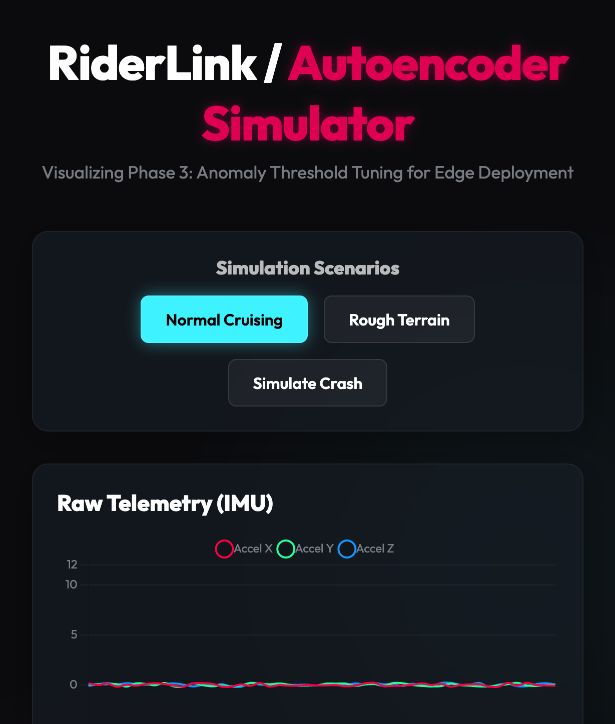
\includegraphics[width=\linewidth]{figures/simulator_normal.jpg}
\par\footnotesize (a) Normal cruising mode with generated traces.
\end{minipage}\hfill
\begin{minipage}[t]{0.48\textwidth}
\centering
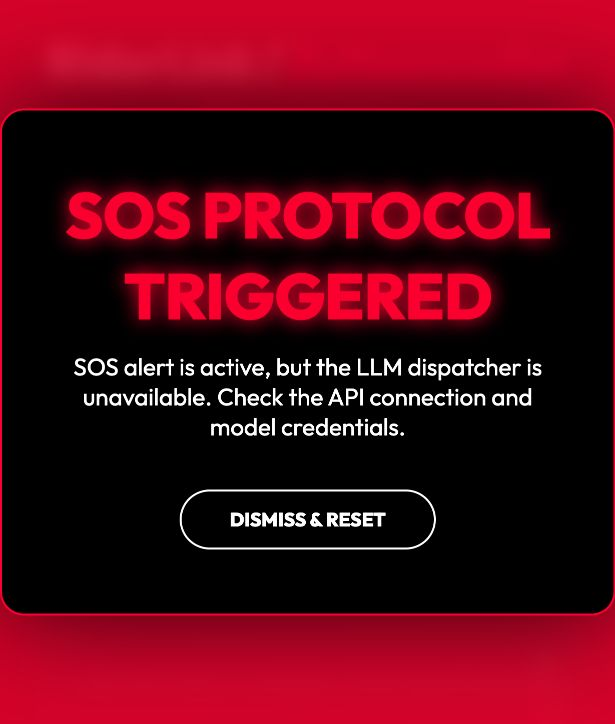
\includegraphics[width=\linewidth]{figures/simulator_crash.jpg}
\par\footnotesize (b) Simulated crash state and SOS interface.
\end{minipage}
\caption{Locally captured RiderLink simulator interface. These screenshots show a software simulation; they do not demonstrate crash detection on a physical motorcycle or emergency-response delivery.}
\label{fig:simulator}
\end{figure*}

\section{Evaluation and Discussion}
This work is an implementation report, not a performance evaluation. The source establishes the presence of a synthetic-data training pipeline, a model export path, an embedded inference wrapper, communications firmware, application-level heuristics, and a browser simulation. It does not provide a reproducible dataset of real rides, a held-out evaluation, a measured confusion matrix, latency, power consumption, memory profile from a compiled target, LoRa range, packet delivery statistics, or end-to-end alert delivery results. Therefore, no accuracy, sensitivity, false-alarm rate, or response-time result is claimed.

A key methodological limitation is the gap between synthetic Gaussian data and realistic motorcycle motion. Road vibration, mounting variation, speed, rider actions, sensor bias, sampling jitter, and near-crash maneuvers can all alter inertial data. The threshold derived from synthetic training errors cannot be assumed to transfer to a physical device. In addition, a dense autoencoder may reconstruct some hazardous events well or flag ordinary maneuvers; both outcomes require empirical testing.

The software boundaries also limit operational interpretation. The simulator does not invoke the trained model, the ESP32 main loop does not invoke the embedded detector, and the mobile app uses a different threshold-based detector. The SOS text service is not a responder dispatch integration. These gaps should be resolved before describing the system as an operational crash detection product.

\section{Limitations and Future Work}
The next research stage should collect consented, labeled, privacy-preserving IMU data across controlled rides, ordinary maneuvers, road conditions, sensor placements, and staged safe impact-like events. A protocol should define sensor units, axes, sampling rate, filtering, window overlap, labeling, and data splits by rider and trip to limit leakage. Thresholds should be selected using training/validation data and assessed on held-out riders and trips. Evaluation should report event-level sensitivity, false alarms per riding hour, precision, detection latency, confidence intervals, and failure cases.

On-device validation should compile and run the wrapper on the target ESP32, record arena use, binary size, inference latency, energy consumption, and behavior under missing or corrupted samples. Integration work should connect a verified detector output to a clear cancellation flow and the LoRa/BLE message format, then exercise packet loss, duplicates, authentication, retries, and offline behavior. Emergency-contact and location handling require explicit user consent, privacy safeguards, and a tested escalation policy. The SOS API should use authenticated, audited integrations before it is represented as dispatch.

\section{Conclusion}
RiderLink is a multi-component motorcycle safety prototype that combines a synthetic-data autoencoder pipeline and TFLite Micro wrapper with ESP32 LoRa/BLE firmware, a Flutter application, a browser simulator, and an optional text-generation service. The repository shows a plausible set of building blocks, but the model is not connected to the ESP32 main program, the simulator does not execute model inference, and the phone application uses a separate heuristic. Because the training data are synthetic and no field evaluation is reported, the current evidence supports a description of implementation only. Real-world data collection, embedded measurement, system integration, and safety-focused validation are necessary before performance or operational safety claims can be made.

\begin{thebibliography}{00}
\bibitem{malhotra2016}
P. Malhotra, L. Vig, G. Shroff, and P. Agarwal, ``LSTM-based encoder-decoder for multi-sensor anomaly detection,'' arXiv:1607.00148, 2016. [Online]. Available: \url{https://arxiv.org/abs/1607.00148}

\bibitem{david2021}
R. David \emph{et al.}, ``TensorFlow Lite Micro: Embedded machine learning for TinyML systems,'' in \emph{Proc. Machine Learning and Systems}, vol. 3, 2021. [Online]. Available: \url{https://proceedings.mlsys.org/paper_files/paper/2021/hash/6c44dc73014d66ba49b28d483a8f8b0d-Abstract.html}

\bibitem{semtech2015}
Semtech Corporation, ``LoRa modulation basics,'' Application Note AN1200.22, Rev. 2, May 2015. [Online]. Available: \url{https://www.semtech.com/uploads/documents/an1200.22.pdf}

\bibitem{riderlink}
A. K. P., ``RiderLink project source repository,'' unpublished project source code, 2026.
\end{thebibliography}
\end{document}
